% !TeX encoding = UTF-8
% !TeX program  = xelatex

\documentclass[12pt,a4paper,openany]{book} 
\usepackage[typeblock=golden]{stb-titlepage}        

%==== Math setup =====================================================
\usepackage{amsmath}%............................. Advanced math (before fonts)
%\usepackage{amssymb}%............................ AMS Symbol fonts

%==== Font setup =====================================================
\usepackage{iftex}
\ifxetex
    \usepackage[math-style=TeX,
                bold-style=TeX,
               ]{unicode-math}
    \setmainfont{Cambria}%........................ Unicode fonts  (Win)                
    \setsansfont[Scale=MatchLowercase]{Calibri}
    \setmonofont[Scale=MatchLowercase]{Consolas}
    \setmathfont{Cambria Math}
    \defaultfontfeatures{Ligatures=TeX}
    \let\bm\symbfit
\else
    \usepackage[utf8]{inputenc}%.................. Unicode file format
    \usepackage{textcomp}%........................ Additional text symbols
    \usepackage[T1]{fontenc}%..................... Type 1 outline fonts
    \usepackage{bm}%.............................. Bold math fonts
\fi
\normalfont

%==== Units and numbers ==============================================
\usepackage{siunitx}%............................. Unit, number and angle output
    \sisetup{detect-all = true, detect-family = true}
    \sisetup{output-decimal-marker = {.} ,
             group-separator = {\,},
             number-unit-product = {\,},
             inter-unit-product = \mathord{\cdot},
             exponent-product = \mathord{\times},
             separate-uncertainty = true}
         
%==== Ref's, Bib's and Nomencl =======================================
\usepackage{stb-nomencl}%......................... List of symbols 
    \renewcommand*{\UnitLabel}[1]{~[\,\unit{#1}\,]}
\usepackage{stb-bib}%............................. Bibliography (natbib internally)
    \bibliographystyle{stb-bib-eng-a}
    \renewcommand\bibfont{\small}
    \renewcommand\bibsection{\chapter{\bibname}}

%==== Tables + Graphics + Color =====================================
\usepackage{array}%............................... Extended table defs 
    \setlength{\extrarowheight}{2pt}
\usepackage{longtable}%........................... Tables can break over pages
\usepackage{graphicx}%............................ Included graphics
\usepackage[font=small]{caption}%................. Customize captions  
\usepackage[table]{xcolor}%....................... Color setup + colortbl 
    
%==== Extra defs for template ========================================
\makeatletter
%---- TOC entries and case
    \renewcommand\contentsname{Table of contents}
    \renewcommand\listfigurename{List of figures}
    \renewcommand\listtablename{List of tables}
    \renewcommand\bibname{List of references}
    
    \renewcommand\tableofcontents{\chapter*{\contentsname}\@starttoc{toc}}
    \renewcommand\listoffigures{\chapter{\listfigurename}\@starttoc{lof}}
    \renewcommand\listoftables{\chapter{\listtablename}\@starttoc{lot}}

%---- Plagiarism signatures
    \newcommand\tstrut[1][4ex]{\rule{0pt}{#1}}
    \newcommand\tdots[1][5cm]{\makebox[#1]{\dotfill}}

%---- Summary head line
    \newcommand\sumheading{%
        \rowcolor[gray]{.9}%
        \centering\arraybackslash%
        \bfseries\normalsize}

%==== User Defs ======================================================
%
% Please insert user defined commands here
% and NOT in the document itself!
%
%
\makeatother

%==== Title Page =====================================================
\title{\textbf{Title}\\[2ex]
       \large Mechatronic Project 478\\Final Report\\[2ex]}                   
\author{\Large Author: Rayde Krüger\\ 
        \large 24723061 \\[5ex]
        \Large Supervisor: Dr. DNJ Els}                
\address{Department of Mechanical and Mechatronic Engineering\\
        Stellenbosch University \\
        Private Bag X1, Matieland 7602, South Africa.}
\date{2023/01/05}                             
\Copyright{2023}{Stellenbosch University.\\ All rights reserved.}

%==== Main Document ==================================================
\setcounter{secnumdepth}{3}
\setcounter{tocdepth}{2}
\raggedbottom
\begin{document}   

\frontmatter%---------------------------------------------------------                    
\maketitle 

\chapter*{Plagiarism declaration}

I have read and understand the Stellenbosch University Policy on Plagiarism and the definitions of plagiarism and self-plagiarism contained in the Policy [Plagiarism: The use of the ideas or material of others without acknowledgement, or the re-use of one's own previously evaluated or published material without acknowledgement or indication thereof (self-plagiarism or text-\-re\-cyc\-ling)].

I also understand that direct translations are plagiarism, unless accompanied by an appropriate acknowledgement of the source. I also know that verbatim copy that has not been explicitly indicated as such, is plagiarism.

I know that plagiarism is a punishable offence and may be referred to the University's Central Disciplinary Committee (CDC) who has the authority to expel me for such an offence.

I know that plagiarism is harmful for the academic environment and that it has a negative impact on any profession.

Accordingly all quotations and contributions from any source whatsoever (including the internet) have been cited fully (acknowledged); further, all verbatim copies have been expressly indicated as such (e.g. through quotation marks) and the sources are cited fully.

I declare that, except where a source has been cited, the work contained in this assignment is my own work and that I have not previously (in its entirety or in part) submitted it for grading in this module/assignment or another module/assignment.
I declare that have not allowed, and will not allow, anyone to use my work (in paper, graphics, electronic, verbal or any other format) with the intention of passing it off as his/her own work.

I know that a mark of zero may be awarded to assignments with plagiarism and also that no opportunity be given to submit an improved assignment. 
\vspace{1.5cm}

\noindent
\begin{tabular}{@{}lllll@{}}
\tstrut Signature: &\tdots&	           &            \\
\tstrut Name:      &\tdots& Student no:&\tdots[3cm] \\
\tstrut Date:      &\tdots&            &            \\
\end{tabular}
		

\chapter*{Executive summary}

\noindent
\begin{longtable}{|p{\dimexpr \linewidth-2\tabcolsep-2\arrayrulewidth}|}
\hline%------------------------------------------------------------
\sumheading  Title of Project \\
\hline%------------------------------------------------------------
 ... \\[1ex]

\hline%------------------------------------------------------------
\sumheading  Objectives \\
\hline%------------------------------------------------------------
 ... \\[1ex]

\hline%------------------------------------------------------------
\sumheading  What is current practice and what are its limitations? \\
\hline%------------------------------------------------------------
 ... \\[1ex]

\hline%------------------------------------------------------------
\sumheading  What is new in this project? \\
\hline%------------------------------------------------------------
 ... \\[1ex]

\hline%------------------------------------------------------------
\sumheading  If the project is successful, how will it make a difference? \\
\hline%------------------------------------------------------------
 ... \\[1ex]

\hline%------------------------------------------------------------
\sumheading  What are the risks to the project being a success? Why is it expected to be successful? \\
\hline%------------------------------------------------------------
 ... \\[1ex]

\hline%------------------------------------------------------------
\sumheading  What contributions have/will other students made/make? \\
\hline%------------------------------------------------------------
 ... \\[1ex]

\hline%------------------------------------------------------------
\sumheading  Which aspects of the project will carry on after completion and why? \\
\hline%------------------------------------------------------------
 ... \\[1ex]

\hline%------------------------------------------------------------
\sumheading  What arrangements have been/will be made to expedite continuation? \\
\hline%------------------------------------------------------------
 ... \\[1ex]

\hline%------------------------------------------------------------
\end{longtable}


\chapter*{Acknowledgements}




% Use \chapter*{} before TOC
\tableofcontents
% Use \chapter{} after TOC

\listoffigures
\listoftables
\chapter{List of symbols}
% Use stb-nomenclature + siunitx

\begin{Nomencl}[1cm]
\NomGroup{Constants}%-----------------------------------------------
    \item[$L_0 = $] \qty{300}{mm}

\NomGroup{Variables}%-----------------------------------------------
    \item[$\mathit{Re}_\mathrm{\,D}$]
                       \UnitLine{Reynolds number (diameter)}{~}
    \item[$x$]         \UnitLine{Coordinate                }{m}
    \item[$\ddot{x}$]  \UnitLine{Acceleration              }{m/s^2}\\
    
    \item[$\theta$]    \UnitLine{Rotation angle            }{rad}
    \item[$\tau$]      \UnitLine{Moment                    }{N.m}

\NomGroup{Vectors and Tensors}%-------------------------------------
    \item[$\overrightarrow{\bm{v}}$] Physical vector, see equation ...

\NomGroup{Subscripts}%----------------------------------------------
    \item[$\mathrm{a}$] Adiabatic
    \item[$a$]          Coordinate

\end{Nomencl}

\begin{Nomencl}[1cm]
\NomGroup{Abreviations}%-----------------------------------------------
    \item[DEM] Discrete Element Method
    \item[FEA] Finite Element Analysis

\end{Nomencl}


\mainmatter%----------------------------------------------------------
\numberwithin{figure}{chapter}
\numberwithin{table}{chapter}

\chapter{Introduction}

\section{Background}

Starting from the big picture, gradually narrow focus down to this project and where this report fits in. Hello world.

\section{Objectives}

The objectives of the project (in some cases the objectives of the report). If necessary describe limitations to the scope.

\section{Motivation}

Why this specific project/report is worthwhile.
\chapter{Literature review}

\section{Discrete element method }

The Discrete Element Method (DEM) analysis \citep{Cundall-1979} uses spherical objects. \citet{Lin:1997} developed a DEM model for ellipsoids.
\chapter{Content chapter}

Unless the chapter heading already makes it clear, an introductory paragraph that explains how this chapter contributes to the objectives of the report/project.

\section{Heading level 2}

\subsection{Heading level 3}

\subsubsection{Deepest heading, only if you cannot do without it}
\vspace{2cm}

\paragraph{Equations:}

An equation must read like part of the text. The solution of the quadratic equation $ax^2+bx+c=0$ given by the following expression (note the full stop after the equation to indicate the end of the sentence):
\begin{equation}
    x = \frac{-b \pm \sqrt{b^2-4ac}}{2b} .
\end{equation}
In other cases the equation is in the middle of the sentence. Then the paragraph following the equation should start with a small letter. Euler's identity is 
\begin{equation}
    e^{i \pi} + 1 = 0 ,
\end{equation}
where $e$ is Euler's number, the base of natural logarithms.

The \texttt{amsmath} has a wealth of structure and information on formatting of mathematical equations.

\pagebreak
\paragraph{Symbols and numbers:}

Symbols that represent values of properties should be printed in italics, but SI units and names of functions (e.g. sin, cos and tan) must not be printed in italics. There must be a small hard space between a number and its unit, e.g. \qty{120}{km}. Use the \texttt{siunitx} package to typeset numbers, angles and quantities with units:
\begin{tabbing}
\hspace*{\parindent}\=\verb|\qty{20}{N.m}|\quad\=$\rightarrow$\quad\=\kill
    \>\verb|\num{1.23e3}| \>$\rightarrow$\> \num{1.23e3} \\
    \>\verb|\ang{30}|     \>$\rightarrow$\> \ang{30} \\
    \>\verb|\qty{20}{N.m}|\>$\rightarrow$\> \qty{20}{N.m}
\end{tabbing}

\paragraph{Figures and tables:}
The \texttt{graphicx} package can import \texttt{PDF}, \texttt{PNG} and \texttt{JPG} graphic files.




\begin{table}[htbp]
    \centering
    \caption{Standard ISO paper sizes}
    \label{tab:paper}
    \begin{tabular}{lcccc}
    \hline
        Paper\quad && \multicolumn{3}{c}{Sizes} \\
    \cline{2-5}
        &&  $W$      && $H$ \\
        && \small [mm] &&  \small [mm]   \\
    \cline{1-1}\cline{3-3}\cline{5-5}
        A0 && 841 && 1189 \\
        A1 && 594 &&  841 \\
        A2 && 420 &&  594 \\
        A3 && 297 &&  420 \\
        A4 && 210 &&  297 \\
        A5 && 148 &&  210 \\
    \hline
    \end{tabular}
\end{table}


\begin{figure}[htbp]
    \centering
    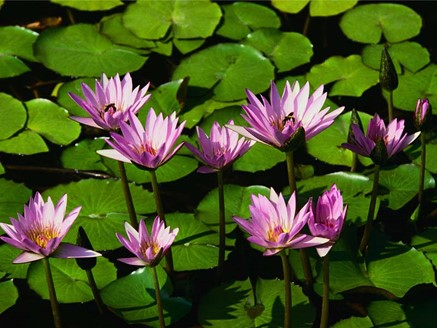
\includegraphics[scale=0.85]{figs/waterplants}
    \caption{Water plants}
    \label{fig:waterplant}
\end{figure}

\chapter{Conclusions}


\appendix%------------------------------------------------------------
\chapter{Mathematical proofs}

\section{Euler's equation}
Euler's equation gives the relationship between the trigonometric functions and the complex exponential function.
\begin{equation}
    e^{ i\theta } = \cos \theta + i\sin \theta
    \label{eq:Euler}
\end{equation}
Inserting $\theta=\pi$ in \eqref{eq:Euler} results in Euler's identity
\begin{equation}
    e^{ i \pi} + 1 = 0
    \label{eq:Euler2}
\end{equation}


\section{Navier Stokes equation}

The Navier–Stokes equations mathematically express momentum balance and conservation of mass for Newtonian fluids.  Navier-Stokes equations using tensor notation:
\begin{subequations}
\begin{gather}
    \frac{\partial \rho}{\partial t} +
    \frac{\partial}{\partial x_j}\left[ \rho u_j \right] = 0 
    \\
    \frac{\partial}{\partial t}\left( \rho u_i \right) +
    \frac{\partial}{\partial x_j}
    \left[ \rho u_i u_j + p \delta_{ij} - \tau_{ji} \right] = 0, \quad i=1,2,3
    \\
    \frac{\partial}{\partial t}\left( \rho e_0 \right) +
    \frac{\partial}{\partial x_j}
    \left[ \rho u_j e_0 + u_j p + q_j - u_i \tau_{ij} \right] = 0
\end{gather}
\end{subequations}

\chapter{Experimental results}


\backmatter%----------------------------------------------------------
\bibliography{bib/bib-sample}
 
\end{document}   

